\chapter{User experience} \label{cha:userexperience}

\section{Basis functionaliteit} \label{sec:basis}
\projectname maakt gebruik van vision om de positie van de wereldbol en de kaart te registreren. De gebruiker moet daarom gemakkelijk deze voorwerpen kunnen gebruiken met zijn/haar handen. De knoppen moeten genoeg van elkaar verspreid staan zodat er geen onhandige situaties ontstaan waarbij de gebruiker per ongeluk knoppen indrukt.\\
In \cref{fig:statemachine1} staat weergegeven hoe de gebruiker navigeert door de applicatie.
\begin{figure}[h]
	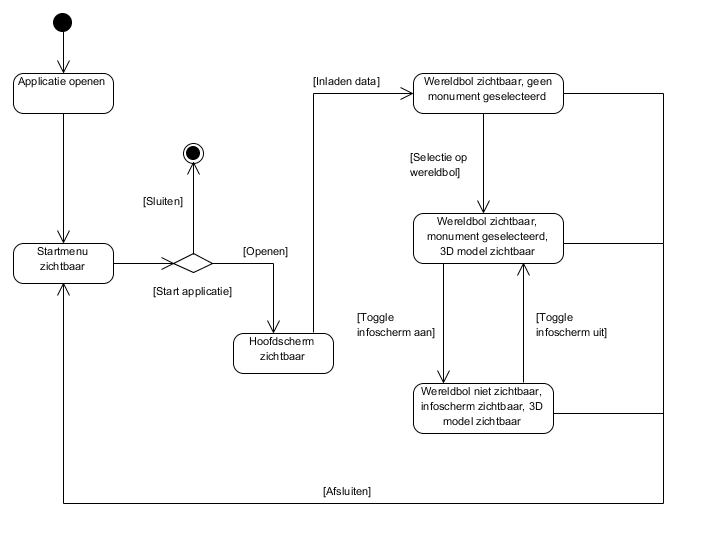
\includegraphics[width=130mm]{figs/state_machine1.png}
	\caption{State Machine diagram userflow}
	\label{fig:statemachine1}
\end{figure}


\newpage
\section{Opstelling} \label{sec:setup}
\begin{figure}[h]
	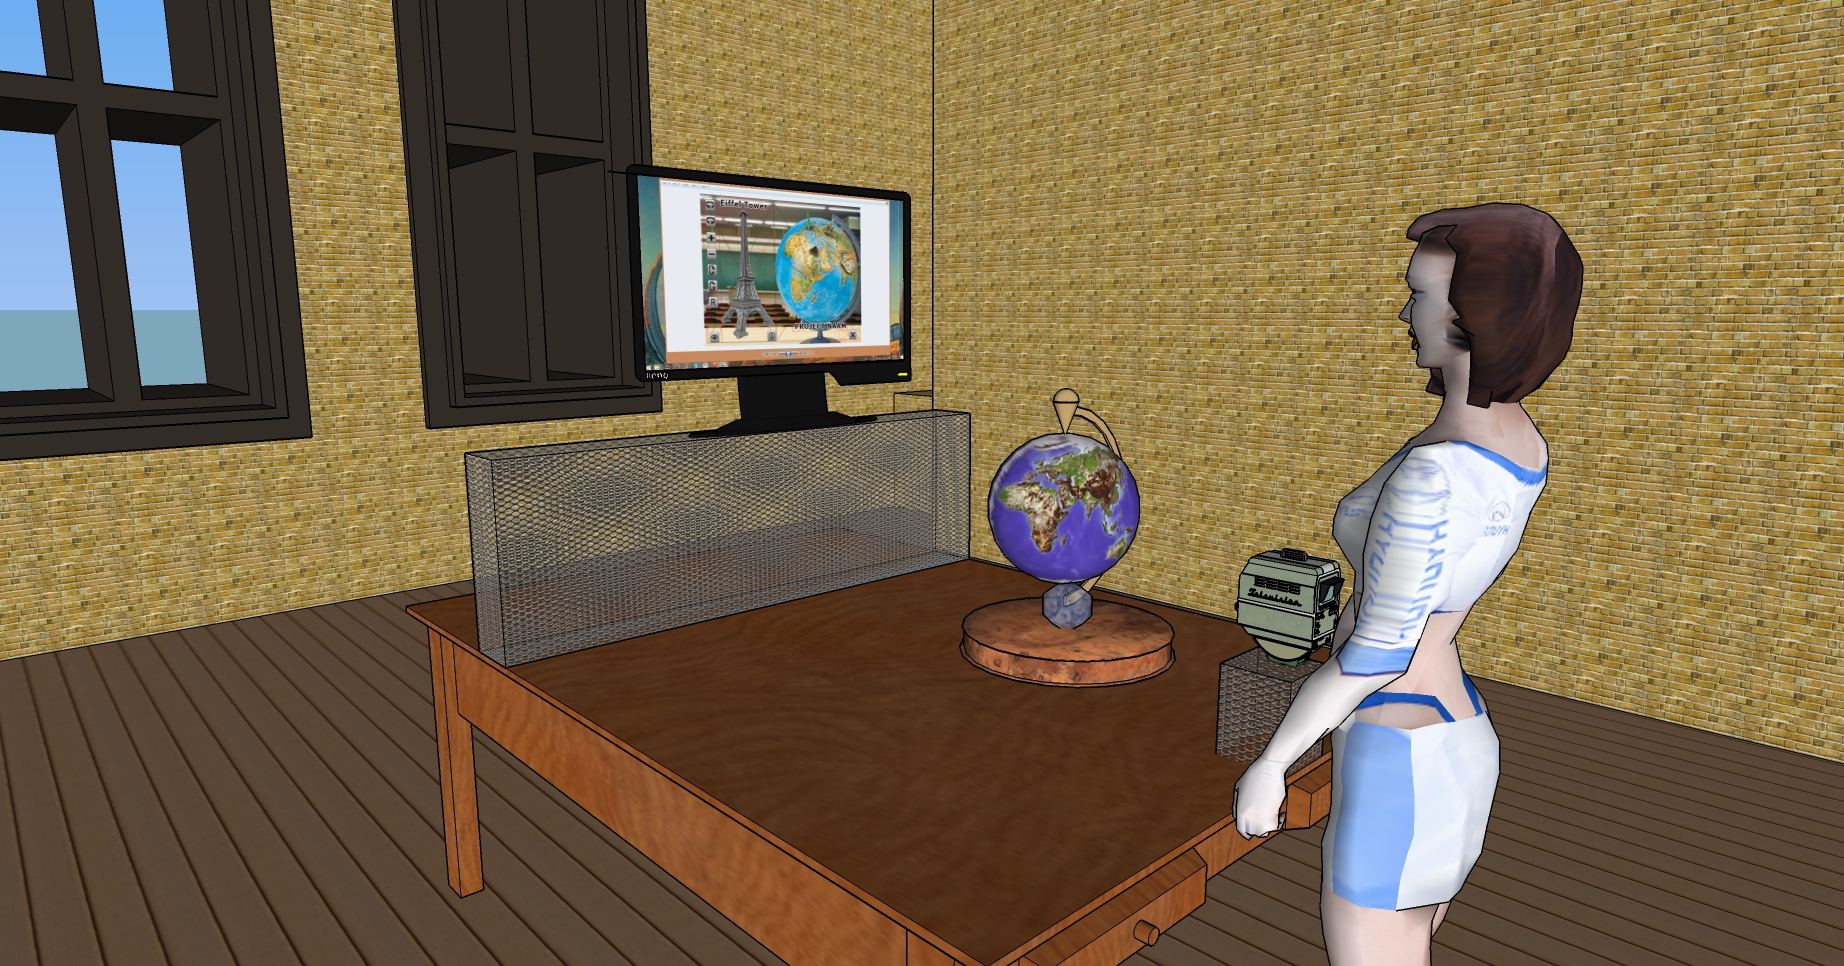
\includegraphics[width=130mm]{figs/screen1.jpg}
	\caption{Fysieke opstelling}
	\label{fig:screen1}
\end{figure}

\begin{figure}[h]
	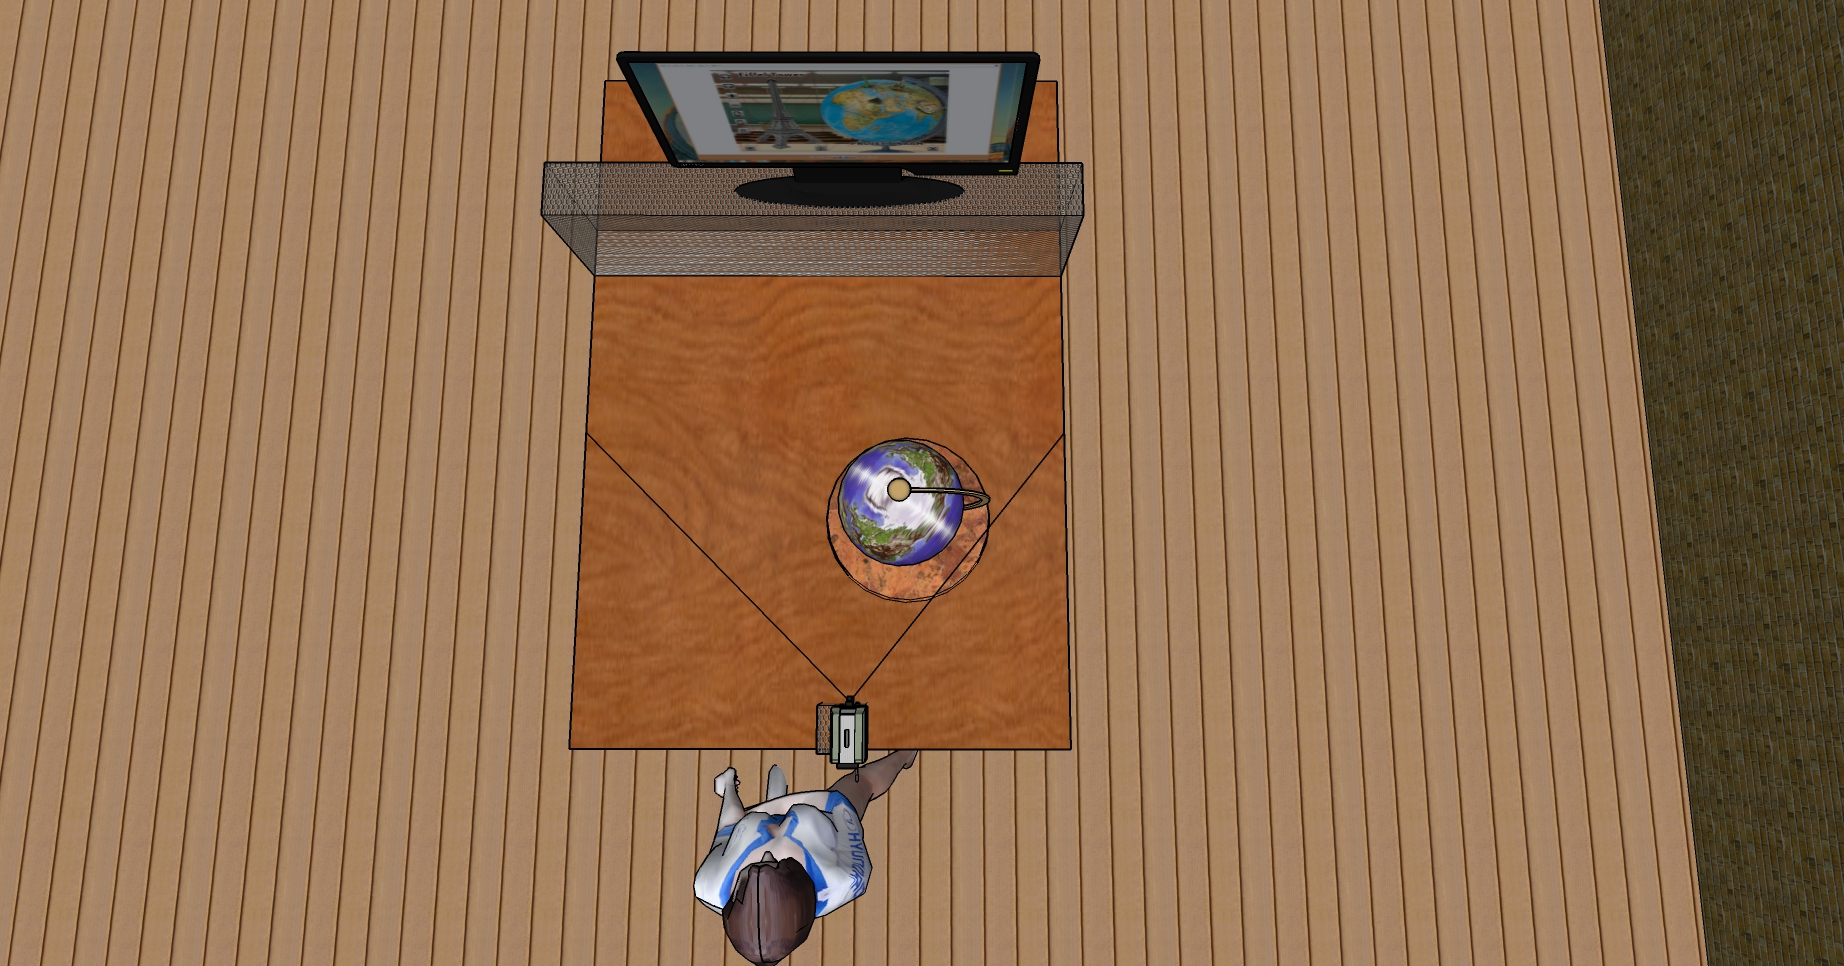
\includegraphics[width=130mm]{figs/screen2.jpg}
	\caption{Fysieke opstelling (topview)}
	\label{fig:screen2}
\end{figure}

Deze concept schetsen (\cref{fig:screen1} en \cref{fig:screen2}) geven het basis idee weer van hoe het gehele product zou moeten worden opgesteld. De camera staat op correcte hoogte om de wereldbol goed weer te geven, maar kan hinderlijk worden ervaren door de gebruiker. De wereldbol staat binnen armlengte van de gebruiker. De camera registreerd de rotatie van de wereldbol en de handen van de gebruiker. Op een computerscherm wordt de applicatie weergegeven, dit scherm wordt verhoogd naar ooghoogte van de gebruiker. Het gehele product moet ergonomisch worden ingericht, nader onderzoek zal worden gedaan naar exacte afmetingen. 
